\documentclass[10pt]{report}
\usepackage[utf8]{inputenc}
\usepackage[top=2cm, bottom=2cm, left=2cm, right=2cm]{geometry}
\usepackage[francais]{babel}
\usepackage{helvet}
\usepackage[T1]{fontenc}
\usepackage{graphicx}
\usepackage{subcaption}
\usepackage{lmodern}
\usepackage{listings}
\usepackage{wrapfig}
\usepackage[colorlinks=true, linkcolor=black, urlcolor=blue, breaklinks, pagebackref, citebordercolor={0 0 0}, filebordercolor={0 0 0}, linkbordercolor={0 0 0}, pagebordercolor={0 0 0}, runbordercolor={0 0 0}, urlbordercolor={0 0 0}, pdfborder={0 0 0}]{hyperref}  %désactive les cadres autour des liens
\usepackage{etoolbox}
\renewcommand{\familydefault}{\sfdefault}

% Supprime l'espace avant l'en-tête des chapitres
\makeatletter
% les chapitres normaux
\patchcmd{\@makechapterhead}{\vspace*{50\p@}}{}{}{}	
% les chapitres étoilés
\patchcmd{\@makeschapterhead}{\vspace*{50\p@}}{}{}{}
\makeatother


\begin{document}

\begin{titlepage}	
	\flushleft
	\begin{figure}[!h]
		
\includegraphics[height=1.8cm]{Reports/figures/logo_insa_cvl.png}
		\hfill
		
\includegraphics[height=3cm]{Reports/figures/logo_biomedia.png}
	\end{figure}
	\centering
	\vspace{2cm}
	{\scshape\Large Stage industriel de 4ème année\par}
	\vspace{1.5cm}
	{\huge\bfseries Développement d'une bibliothèque mathématique performante pour le traitement d'images médicales\par}
	\vspace{2cm}
	{\Large\itshape Élève ingénieur: François PIAT\par}
		\vspace{1cm}
	\begin{figure}[!h]
		\begin{center}
			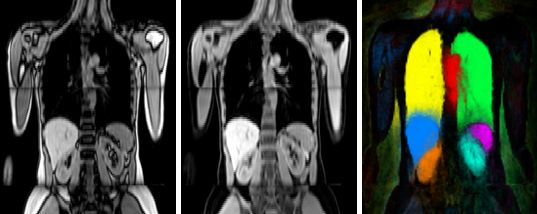
\includegraphics[width=13cm]{Reports/figures/biomedia_image.png}
		\end{center}
	\end{figure}
	\vfill
	\flushleft
	Tuteur INSA: \hfill Tuteurs BioMedIA: \par
	Dr. Julien \textsc{Olivier} \hfill Dr. Ghislain-Anthony \textsc{Vaillant} \\ \hfill Dr. Jonathan \textsc{Passerat-Palmbach}
	\vfill
	% Bottom of the page
	\centering
	{\large Année universitaire 2015 - 2016 \par}
\end{titlepage}

\section*{Remerciements}\newpage
\paragraph*{Résumé} % dans cet ordre
\paragraph*{Mots-clés}
\paragraph*{Abstract}
\paragraph*{Key-words}

\renewcommand\contentsname{Sommaire}
\tableofcontents

\newpage

\chapter*{Introduction}
\addcontentsline{toc}{chapter}{Introduction}

\chapter{Environnement de travail} 

	Le stage s'inscrivant dans un cadre de recherche, cette section présente le laboratoire dans lequel il s'est déroulé.
	\section{Le laboratoire}
	\subsection{Imperial College London - Department of computing}
	\paragraph{Imperial College London}~\par ~\par %souligner la section ou l'on est
	L’Imperial College London (officiellement The Imperial College of Science, Technology and Medicine) est une université britannique fondée en 1907 par la fusion du City and Guilds College, de la Royal School of Mines et du Royal College of Science (tous fondés entre 1845 et 1878).\\ ~\par
    L'université possède au total 9 campus, tous situés à Londres, et dont la plupart sont implantés dans des sites hospitaliers.  
    Elle possède 5 départements administratifs et 4 branches techniques: ingénierie, sciences naturelles, business, et médecine.	Le campus principal est basé dans le quartier du South Kensington, et regroupe la branche d'ingénierie, de sciences naturelles, d'arts et de business. C'est sur ce campus que le département d'informatique est donc basé. 
    
	\begin{figure}[h!]
		\begin{center}
			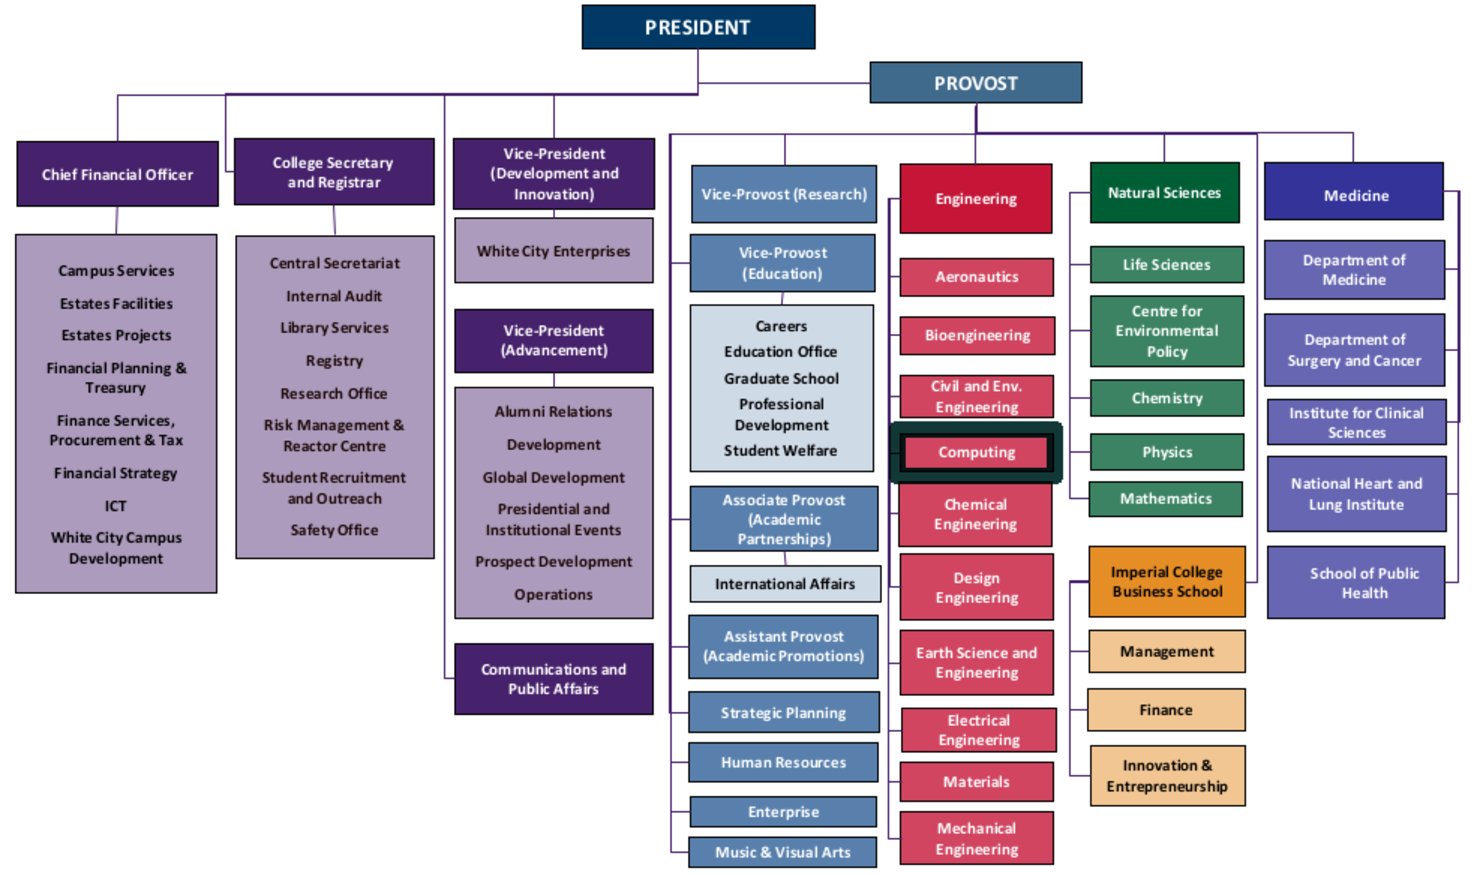
\includegraphics[width=18cm]{Reports/figures/College-Organisation.pdf}
		\end{center}
		\caption{Organigramme de l'Imperial College London \\ \textit{Le département de computing, encadré en noir, se situe dans la branche d'ingénierie (en rouge) de l'université.}}
		\label{Organigramme de l'Imperial College London}
	\end{figure}
	
	\paragraph{Department of computing}~\par~\par
	
	Le département d'informatique est divisé en 5 groupes de recherche : 
	\\{$\bullet$}\textit{\textbf{Logic and Artificial Intelligence:}} la recherche en Logic and Artificial Intelligence englobe des études fondamentales de logique et une variété de disciplines en intelligence artificielle.
	\\{$\bullet$}\textit{\textbf{Distributed Software Engineering:}}	la recherche dans le domaine du Distributed Software Engineering aborde la conception de systèmes distribués, adaptatifs et fiables.
	\\{$\bullet$}\textit{\textbf{Quantitative Analysis and Decision Science:}} la recherche en Quantitative Analysis and Decision Science varie de l'optimisation à l'ingénierie de performances, en passant par la des expériences de vérifications quantitatives ou de sécurité.
	\\{$\bullet$}\textit{\textbf{Programming Languages and Systems:}} Programming Languages and Systems est une section qui combine des travaux théoriques et pratiques en langages et architecture pour obtenir des logiciels rapides, et efficaces.
	\\{$\bullet$}\textit{\textbf{Visual Information Processing:}} la recherche en Visual Information Processing couvre une multitude de domaines, incluant la vision numérique, les graphiques, l'apprentissage automatique, et le traitement d'images médicales.
	 
	\begin{wrapfigure}[13]{r}{10cm}
		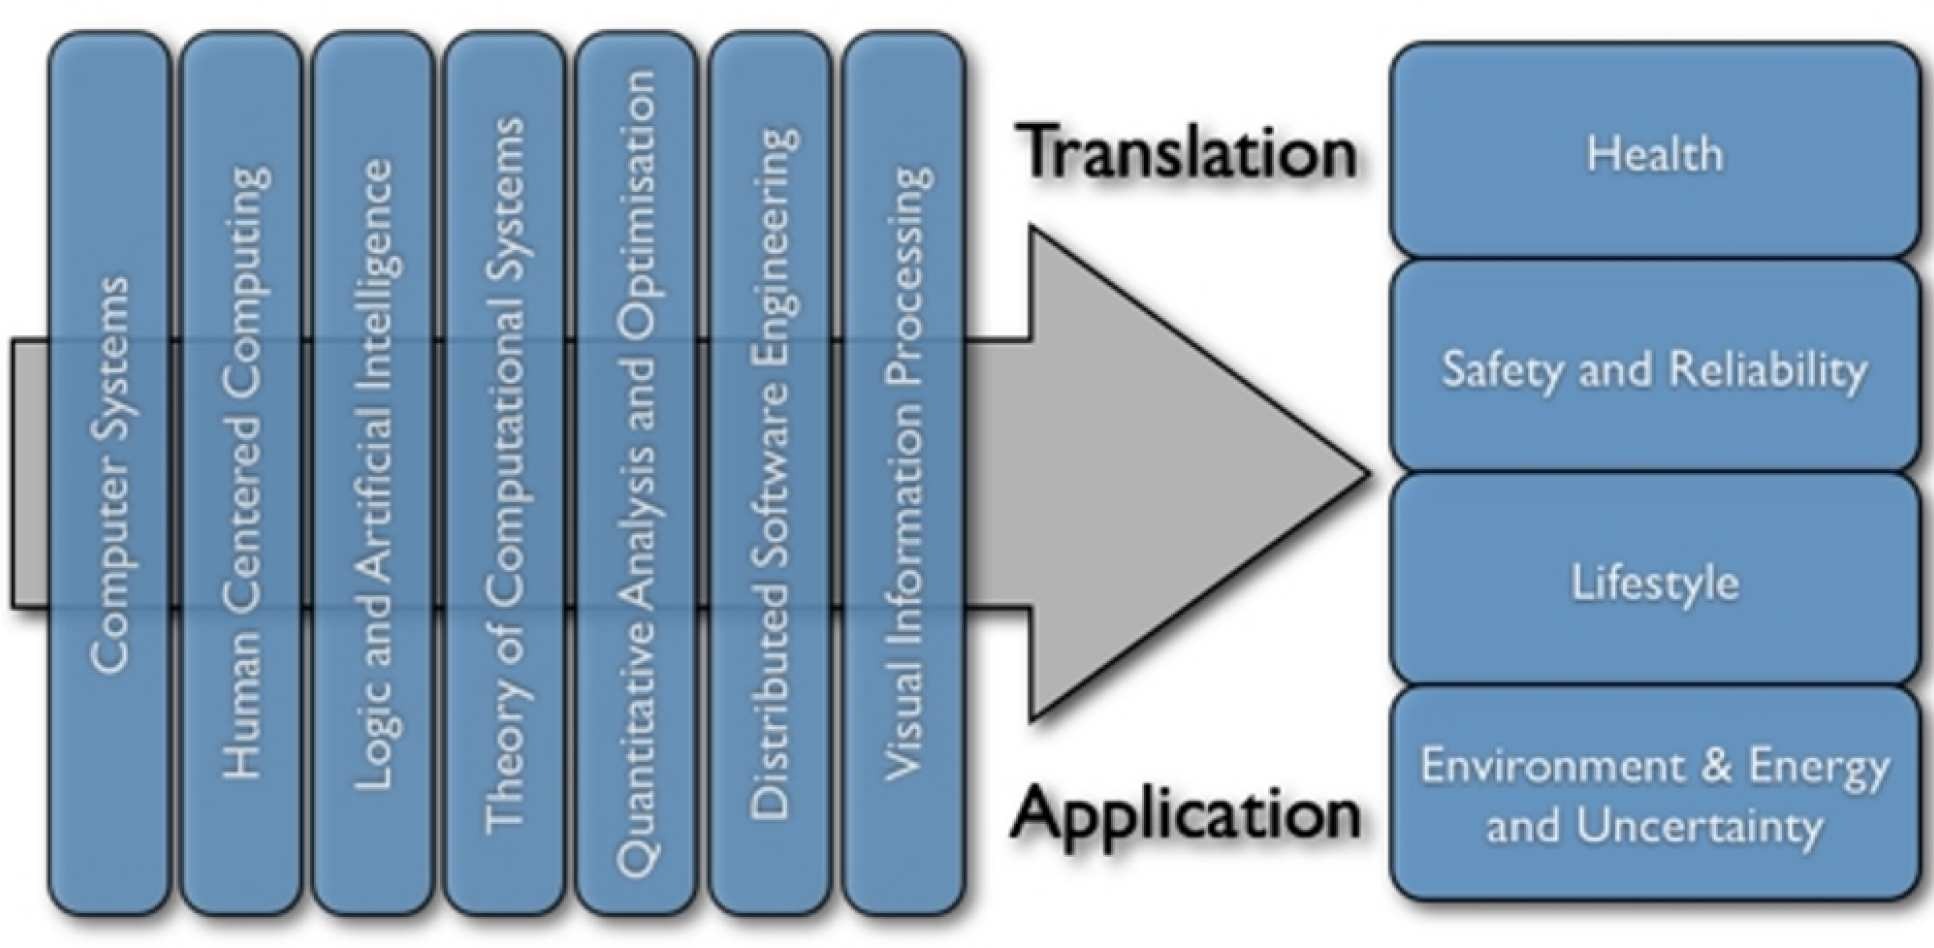
\includegraphics[width=9cm]{Reports/figures/research_strategy.jpg}
		\caption{Stratégie du département de recherche}
		\label{Stratégie du département de recherche}
	\end{wrapfigure}~\par~\par
	
	Les différentes spécialités citées précédemment sont articulées au sein du centre de recherche afin d'appliquer les résultats à d'autres domaines de recherche. Ces principales applications concernent les domaines de la santé, de la fiabilité/sécurité, de l'environnement, des modes de vie, de l'énergie et des incertitudes.
	\\
	\\
	\subsection{BioMedIA}

	La mission du groupe BioMedIA est de développer de nouvelles techniques de
	calcul pour l'analyse d'images biomédicales. Le groupe se concentre sur des
	domaines de recherche de pointe, y compris:\\
	{$\bullet$} Le développement d'algorithmes d'acquisition, d'analyse et d'interprétation des images. En particulier dans les domaines du recalage, de la reconstruction,
	du suivi de mouvement, de la segmentation et de la modélisation. \\
	{$\bullet$} L'apprentissage machine pour l'extraction d'information clinique à partir
	d'images médicales. Les applications incluent le diagnostic assisté par
	ordinateur, la planification automatisée de traitement médical, ou encore la thérapie et les interventions guidées par ordinateur. \\
	Le laboratoire s'intéresse particulièrement à l'imagerie et les technologies de
	traitement informatique qui permet de mieux comprendre le
	développement du cerveau humain, l’évolution des maladies mentales et le
	diagnostic des patients atteints de maladie cardiovasculaire.
	
	\section{Cadre du projet} 
	\subsection{Medical Image Registration Toolkit (MIRTK)}~\par~\par
	Le Medical Image Registration Tool-Kit (abrégé MIRTK) est un logiciel open-source de traitement d'images médicales codé en C++ et utilisé par des chercheurs dans le milieu médical. Ces chercheurs sont, grâce à ce logiciel, aptes à analyser et manipuler des images en 2,3 ou 4 dimensions. \\ 
	L'utilisation de MIRTK est basée sur l'appel de lignes de commandes, incluant le nom de la fonction, les paramètres et les arguments nécessaires, et propres à chacune des fonctions. Par exemple, la ligne de commande suivante va rogner une image :
	
	\begin{lstlisting}
mirtk extract-image-region input.nii.gz output.nii.gz -Rx1 50 -Rx2 40 -Ry1 250 -Ry2 250
	\end{lstlisting}
	
	Sur cette ligne de commande:
	\\{$\bullet$} "mirtk" indique que l'on souhaite utiliser une fonction de MIRTK
	\\{$\bullet$} "extract-image-region" appelle la fonction de rognage
	\\{$\bullet$} "input.nii.gz" indique l'emplacement de l'image d'entrée, idem pour la sortie avec "output.nii.gz". Ces fichiers sont au format NIFTI (ici, ces images sont aussi compressées), seul format pris en charge par MIRTK.
	\\{$\bullet$} "-Rx1 50" signifie "retirer 50 pixels sur l'axe x, pour la première direction" (idem pour "-Rx2 40 -Ry1 250 -Ry2 250"). 
	L'action de cette ligne de commande est visualisable sur la Figure \ref{Effet de la fonction "extract-image-region"}.
	
	\begin{figure}[h!]
		\centering
		\begin{subfigure}{.5\textwidth}
			\centering
			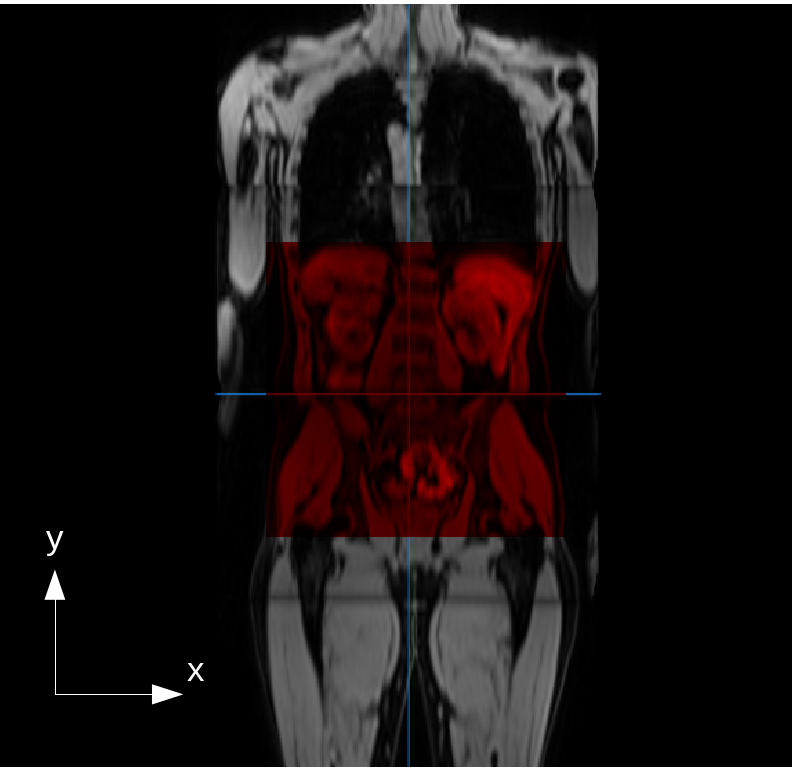
\includegraphics[width=5cm]{Reports/figures/mirtkextractregion1d.png}
			\caption{Image d'entrée}
			\label{Image d'entrée}
		\end{subfigure}%
		\begin{subfigure}{.5\textwidth}
			\centering
			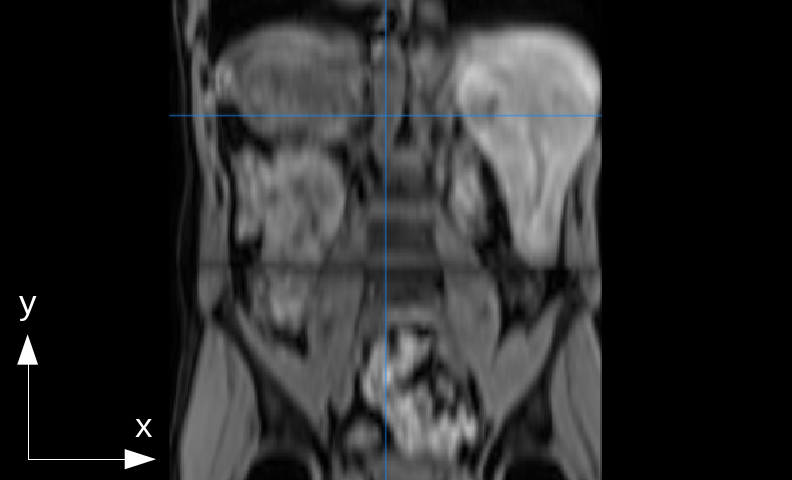
\includegraphics[width=7cm]{Reports/figures/mirtkextractregion2_1d.png}
			\caption{Image de sortie}
			\label{Image de sortie}
		\end{subfigure}
		\caption{Effet de la fonction "extract-image-region"}
		\label{Effet de la fonction "extract-image-region"}
	\end{figure}~\par
	
	Chaque fonction de MIRTK est exécutée par un fichier binaire qui a été généré par le fichier d'application associé. Tous ces fichiers sont d'ailleurs répertoriés dans un dossier \textit{Applications} et font appel à certaines dépendances, qui sont réparties en 7 modules : \textit{Common, Image, I/O, Numerics, PointSet, Registration} et \textit{Transformation}. Ces différents modules représentent le lien entre le back-end de MIRTK et son corps. Le recalage d'image (Registration) est l'une de ses principales fonctions.
	
	 \subsection{UK BioBank}~\par
	 "UK BioBank" est le nom donné à un projet initié par plusieurs entités de recherche du Royaume-Uni . En collaboration avec le gouvernement britannique, ce projet prévoit de regrouper la plus grosse banque de données médicales du Royaume-Uni. En plus de données numériques, cette base de données regroupera aussi des dizaines de données extra-médicales pour chaque patient. Ceci pourrait permettre, après analyse, de pouvoir corréler des comportements individuels communs à une ou plusieurs maladies graves. ~\par~\par
	 
	 MIRTK à le potentiel pour s'inscrire dans ce projet, à long terme, en tant que "boite à outils" officielle, permettant d'analyser et d'étudier les grandes quantités de données visualisables de UK BioBank. ~\par~\par
	 Le projet de UK BioBank compte obtenir des données relatives à 100 000 individus. Parmi ces données seront inclues des images médicales qu'il faudra analyser. A l'heure actuelle, MIRTK est adapté pour manipuler quelques dizaines de ce type d'images, mais à besoin d'une amélioration de ses performances. Dans ce cadre, le but principal de ce stage est donc de commencer la démarche d'amélioration du logiciel en terme de design et de performances.
	 
\chapter{Objectifs et cahiers des charges}

	\section{Problématique} 
	Dans l'optique de préparer MIRTK à son insertion dans le projet UK BioBank, et d'obtenir des résultats concluant relativement rapidement, on pourra distribuer les calculs à différentes échelles : \\
	\t - sur un slurm, qui correspond a un réseau local de machines.\\
	\t - sur un High Performance Computing (HPC), qui s'étant à tous le réseau de machines de l'Imperial college, mais qui est un service payant.\\
	\t - sur un cloud, soit un serveur que l'on loue à une entreprise qui propose un tel service, telles que Google ou Amazon.\\ ~\par
	Ces différents supports de calculs pourront accélérer l'obtention des résultats, sachant que la liste précédente est classée de manière croissante concernant la rapidité d'exécution. Cependant, le HPC ou un cloud serait payant, avec un prix croissant selon le temps d'exécution. Semblablement, un slurm utilise les performances d'autres machines, qui, elles-même peuvent éventuellement être déjà occupées par l'exécution d'un autre logiciel. C'est pourquoi une exécution de MIRTK devra être la plus rapide possible, puisque, dans tous les cas, elle sera répétée un grand nombre de fois sur le support choisi.
	\vspace{-0.5cm}
	
	\begin{wrapfigure}[20]{r}{9cm}
		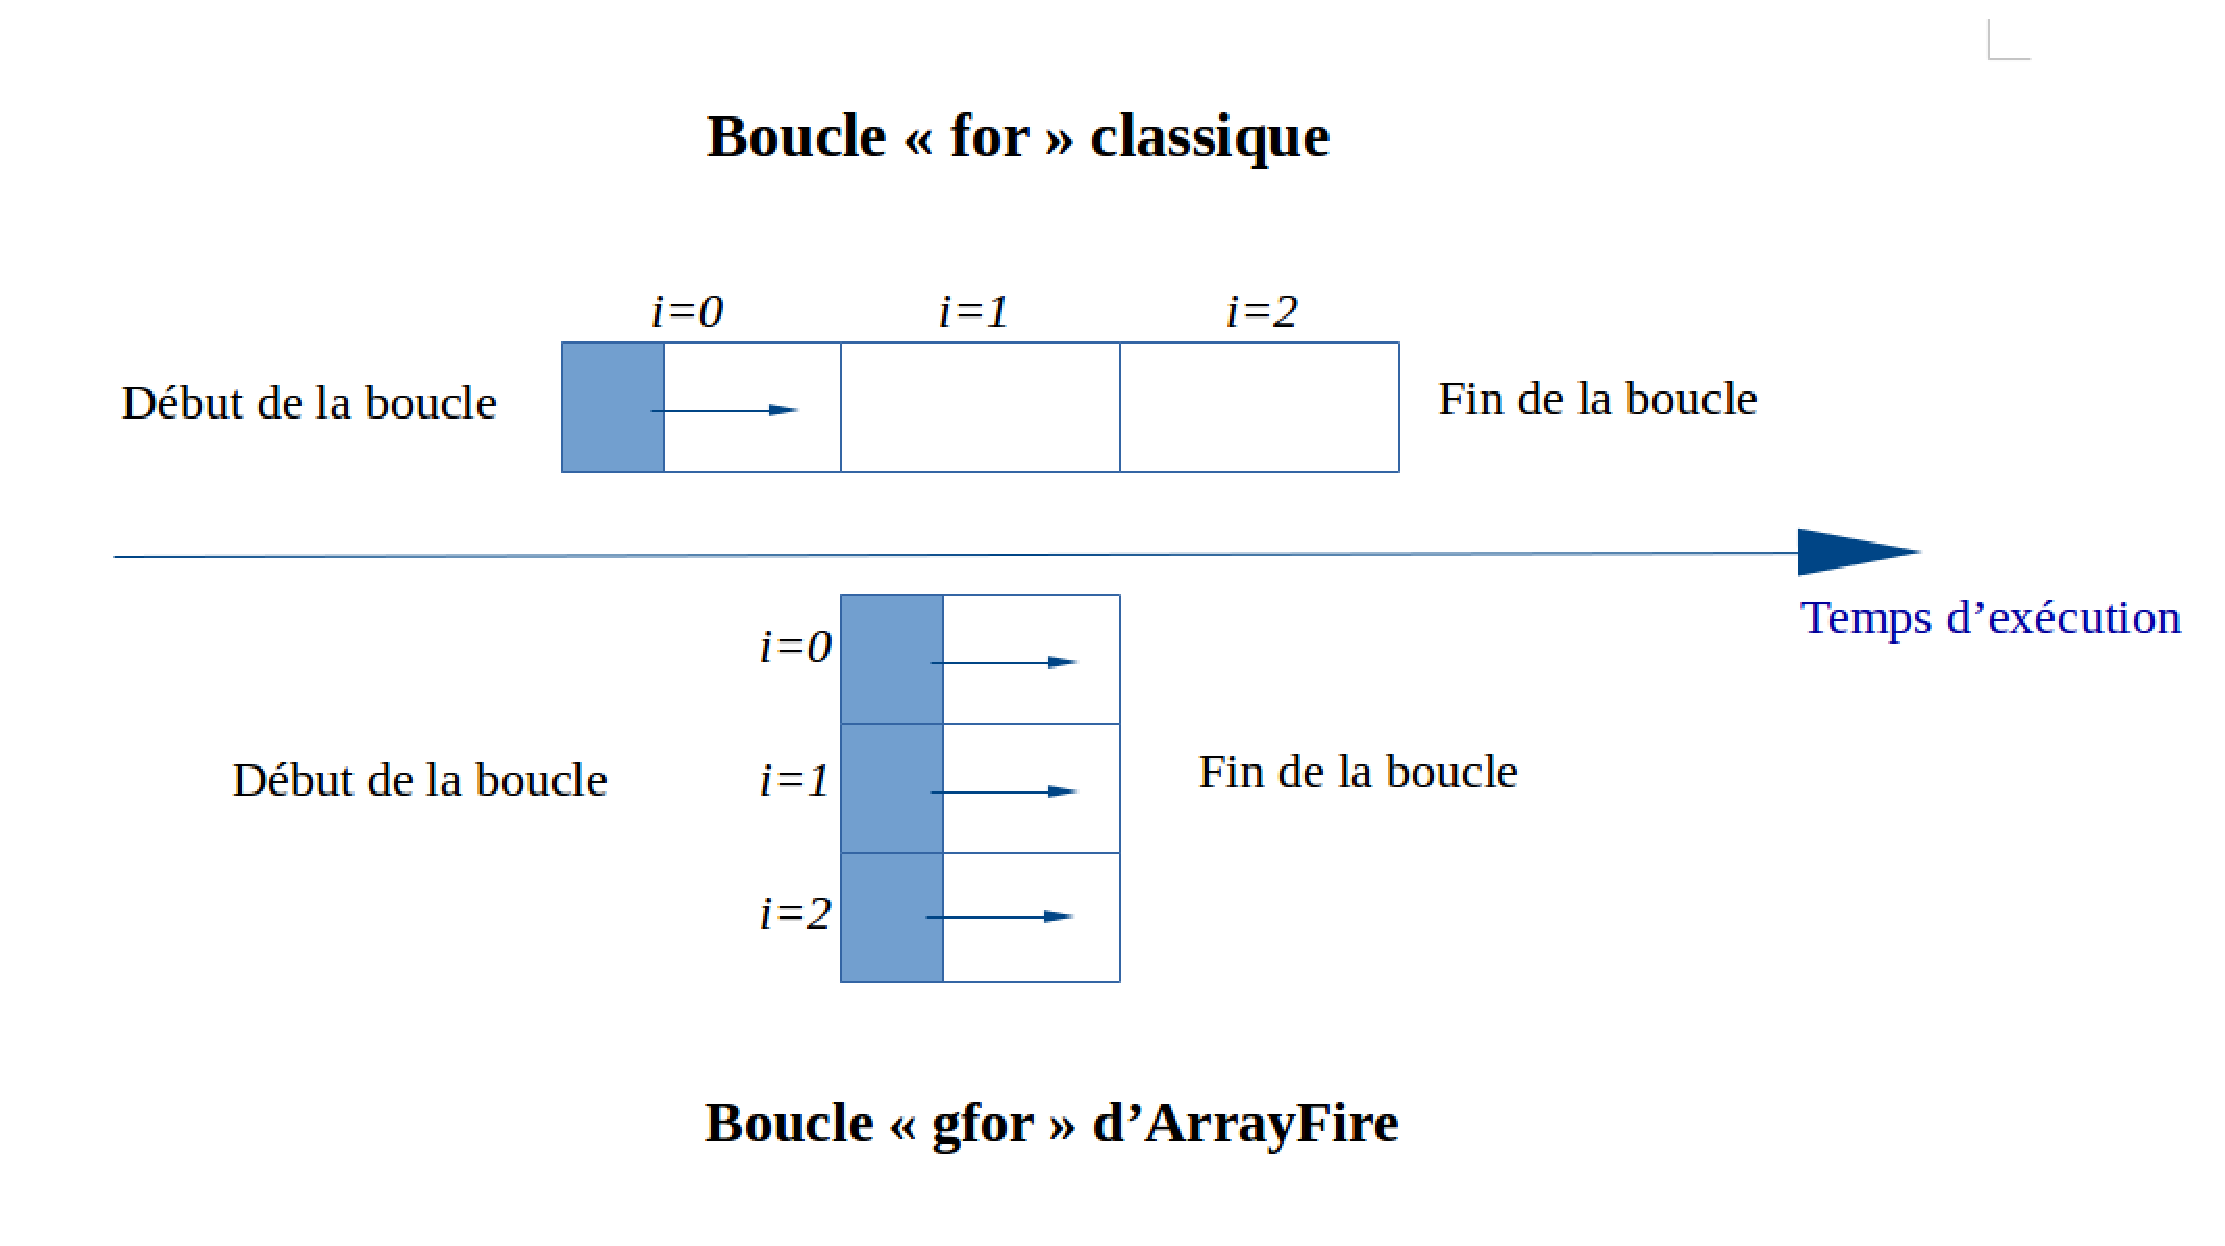
\includegraphics[width=10cm]{Reports/figures/gfor.eps}	
		\caption{Fonctionnement d'une boucle en parallèle}
		\label{Fonctionnement d'une boucle en parallèle}
	\end{wrapfigure}
	
	~\par~\par
	Par conséquent, le secteur sur lequel il faudra se pencher sera donc la réduction du temps d'exécution des fonctions du logiciel. Pour cela, MIRTK utilise une technique d'optimisation appelée "la parallélisation" d'un code. A l'inverse de l'exécution sérialisée, le principe de la parallélisation est d'assigner plusieurs threads dédiés à la commande appelée. Une fois assignés, chaque thread reçoit une quantité de "blocks" de code a exécuter. Chaque thread pourra donc traiter un block indépendamment du reste de l'exécution. Ainsi, plus la quantité de threads utilisée est grande, plus l'exécution sera accélérée. La figure \ref{Fonctionnement d'une boucle en parallèle} ci-contre représente ce principe avec des blocks de 2 itérations.\\

	La problématique du stage s'axera sur une optimisation de MIRTK au niveau des couches logicielles de bas niveau. Le logiciel, pour opérer chacune de ses fonctions, fait appel des dépendances mathématiques, implémentées dans le module \textit{Numerics}. La majeure partie du stage concernera donc ce module de MIRTK, c'est-à-dire les fonctions utilisant majoritairement des opérations matricielles.\\
	
	\section{Cahier des charges}
	La réduction du temps d'exécution est l'objectif principal du stage. Pour cela, il va falloir travailler sur 3 plans principaux : \\
	\\{$\bullet$} La compatibilité avec différents back-end, que ce soit pour processur (CPU) ou carte graphique (GPU). A l'heure actuelle, la gestion des back-end GPU n'est pas assurée par le logiciel. Le rendu idéal serait de laisser MIRTK gérer automatiquement cet aspect, en vérifiant la présence d'une carte graphique sur l'ordinateur (sinon utiliser le CPU), puis le laisser choisir entre CPU et GPU pour des performances optimales. Si, par exemple, un ordinateur possède une bonne carte graphique, MIRTK devra être apte à le détecter, et donc de l'utiliser.\\
	\\{$\bullet$} Garder l'intégrité et la transparence du code de MIRTK. Il sera imposé de garder les mêmes fonctions (ainsi que leurs arguments) et la même API. Pour conserver cela, il faudra garder une transparence entre le code de MIRTK et la gestion de différents back-end. C'est-à-dire que l'implémentation la plus haut niveau des fonctions du logiciel devra rester inchangée.\\
	\\{$\bullet$} Dans la mesure du possible, les fonctionnalités qui auront été dupliquées pendant le stage devront être supprimées, avec idéalement, la suppression d'une ou plusieurs dépendances du logiciel.
	
	\section{Stratégie employée}
	\subsection{Objectifs} 
	Afin de se familiariser avec MIRTK, les objectifs ont été établis de manière chronologique, de la manière suivante: 
	~\par~\par 
	1) \textbf{Études de MIRTK et de ses dépendances, et analyse de l'API d'ArrayFire} \\
	Cette étape préliminaire permettra de comprendre le fonctionnement global de MIRTK et de se familiariser avec son code source. Dans le même temps, l'analyse de l'interface d'ArrayFire, et des différentes fonctions proposées par la bibliothèque. Cette étude corrélera donc les besoins de MIRTK et les solutions proposées par ArrayFire.
	~\par~\par 
	2) \textbf{Profilage de MIRTK}\\
	Afin d'obtenir une première visualisation des performances du logiciel, un profilage sera exécuté sur les fonctions concernées. L'interprétation de ces premiers résultats sera nécessaire pour élaborer un ordre de priorité dans les fonctions à ré-implémenter.
	~\par~\par 
	\t 3) \textbf{Intégration de ArrayFire dans MIRTK} \\
	A la suite du profilage sera donc obtenue une liste de fonctions à implémenter primordialement. La modification de ces fonctions sera faite indépendamment, en commençant par les fonctions dont la ré-implémentation sera la plus simple, en progressant ensuite sur celles plus complexes.
	~\par~\par
	\t 4) \textbf{Implémentation de la gestion optimisée des back-ends} \\
	Afin d'apporter une fonctionnalité davantage liée au hardware utilisé, la gestion des back-ends serait un avantage pour les performances de MIRTK. Pour cette raison, cette gestion sera idéalement implémentée en fin de stage. 
	~\par~\par 
	\t 5) \textbf{Benchmarking} \\
	Pour prouver l'efficacité d'ArrayFire et l'amélioration des performances de MIRTK, un test des fonctions précédemment optimisées sera réalisé. Les résultats attendus sont principalement des graphiques reflétant cette amélioration.
%	Détailler les objectifs a atteindre idéalement.
%	- Ajouter ArrayFire à MIRTK, en remplaçant les fonctions d'EIGEN les moins adaptées par les fonctions d'AF. \newline
%	- Faire un profiling des fonctions concernées par TBB, et interpréter les résultats afin d'élaborer une stratégie pour implanter la programmation // d'AF.\newline
%	- Supprimer les TBB inutiles ou peu efficaces, et remplacer les autres par l'équivalent d'AF (gfor).\newline
%	\noindent Dans un premier temps, il faudrait analyser le code de MIRTK sur deux plans:\\~\par 
%	\t - Les fonctions utilisées par Eigen et qui seraient davantage adaptées avec ArrayFire \\~\par
%	\t - Les outils de parallélisation et l'utilisation de la bibliothèque TBB \\\\
%	La première étape se fera simplement en comparant l'utilisation directe de Eigen, ainsi que les interdépendances des fichiers MIRTK avec ceux de la bibliothèque. Cependant, la deuxième demandera une analyse plus approfondie: en plus d'une analyse de code tel que précédemment avec EIGEN, il faudra réaliser un "test de performance" sur certaines fonctions. Ce test est appelé un profilage (ou \textit{profiling} en anglais) et peut analyser différents critères. Ainsi pourrons-nous cibler les fonctions les plus urgentes à modifier, qui sont mal rédigées ou qui demande relativement trop de ressources.
%	A la suite de ce profilage sera donc élaboré un "plan d'attaque" pour savoir par quelle partie du projet commencer.
%	\t - A terme, après avoir retiré au maximum les dépendances de MIRTK avec TBB, on pourra commencer des tests de benchmarking afin de vérifier l'amélioration des performances.
	\subsection{Diagramme de GANTT}
%	 => gantt chart prévisionnel (à mettre en français)
%	\begin{figure}[h!]
%		\begin{center}
%			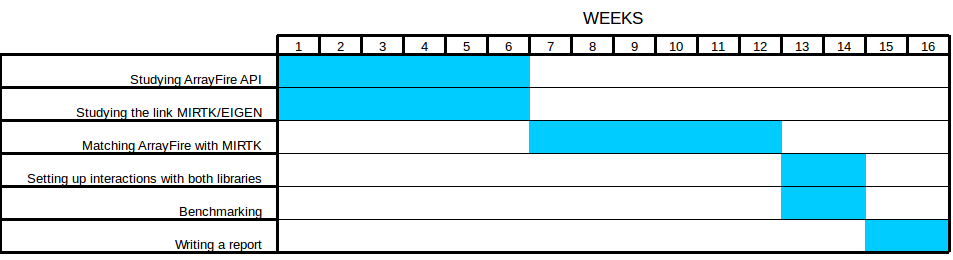
\includegraphics[width=18cm]{Reports/figures/estimated_gantt.png}
%		\end{center}	
%		\caption{Diagramme de GANTT prévisionnel}
%		\label{Diagramme de GANTT prévisionnel}
%	\end{figure}
\chapter{Réalisation}
	\section{Choix et justification du module mathématique}

	
	\section{Implémentation}
	\subsection{Intégration du module mathématique} 
	%	Programmation transparente entre Eigen et ArrayFire.
	%	Lister les fonctions principales à substituer.
	
	% A refaire !!!!
%	L'une des premières fonctions qui nous a attiré était un filtre, qui avait une implémentation assez simple (un simple produit de convolution de deux matrices). On a donc choisi de s'y intéresser avec ArrayFire.
%	Ce filtre a été précédemment profilé, il s'agit de la fonction \textit{smooth-image}. La version de MIRTK était déjà implémentée de manière séparable, c'est-à-dire que le floutage est réalisé une dimension après l'autre, et c'est la méthode la plus optimisée pour un tel calcul. Cependant, on a tout de même remplacé l'implémentation existante en intégrant ArrayFire afin de comparer les performances et simplifier le code de la fonction. \\
%	Dans un premier temps, une implémentation naïve a été initiée en reprenant à zéro le code de la fonction. Le floutage d'une image se fais par un produit de convolution entre la matrice représentant l'image, et le filtre (gaussien), qui est déclaré dans la fonction elle-même. L'implémentation naïve a donc été de réaliser ce produit de convolution de matrices en utilisant la fonction \textit{af::convolve}, qui réalise simplement la convolution du filtre 3D avec l'image 3D, comme on peut le voir ci-dessous:\\
%	\begin{figure}[h!]
%		\begin{center}
%			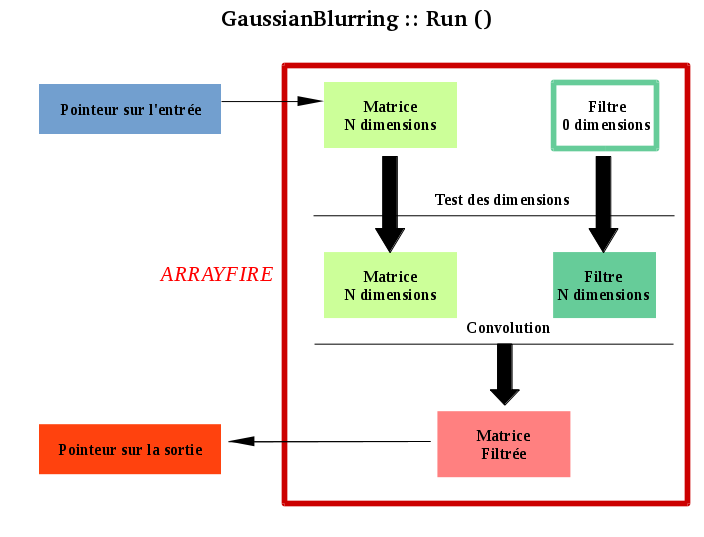
\includegraphics[width=11cm]{Reports/figures/gaussianblurring.png}
%		\end{center}	
%		\caption{Algorithme de flou gaussien incluant Arrayfire - Implémentation naïve}
%		\label{Algorithme de flou gaussien incluant Arrayfire - Implémentation naïve}
%	\end{figure}~\par
%	Afin d'optimiser au maximum la fonction, il faut maintenant la ré-implémenter de la même manière que dans MIRTK, c'est-à-dire de manière séparable. Pour cela on effectue sur chaque dimension un produit de convolution sur la dimension 1 de la matrice, qu'on réordonne après, de telle manière à faire passer les valeurs de la dimension choisie en première dimension: \\
%	\begin{figure}[h!]
%		\begin{center}
%			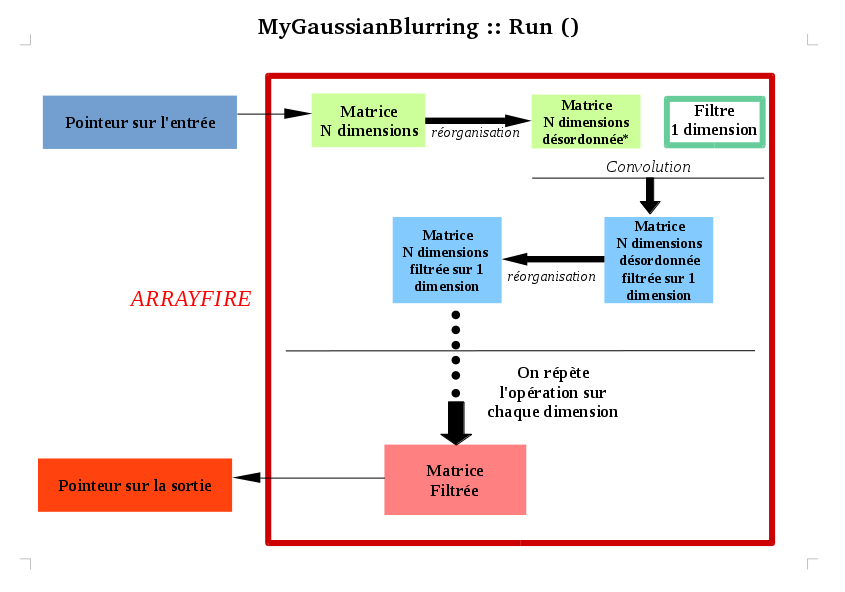
\includegraphics[width=12cm]{Reports/figures/mygaussianblurring.png}
%		\end{center}	
%		\caption{Algorithme de flou gaussien incluant Arrayfire - Implémentation optimisée}
%		\label{Algorithme de flou gaussien incluant Arrayfire - Implémentation optimisée}
%	\end{figure}~\par
	\subsection{Dette technique}
	%	Optimisation des threads et suppression de TBB au profit de ArrayFire.
	
	
	
	
	%	\newline
	%	Le contenus des sous-parties, ainsi que d'éventuelles d'autres sous-parties dépendront du résultat du profilage.
	
	\section{Analyse des performances}
		\subsection{Profilage}
	%	Définir le profilage et expliquer la nécessité d'une telle étape dans ce contexte\newline
	
		% a refaire!!!
%		Lors du début de mon stage, il a fallu que je me familiarise avec les dépendances de MIRTK, mais aussi a son fonctionnement interne. C'est lors de cette étude préliminaire que mon tuteur et moi avons étudié, en plus de la bibliothèque EIGEN (destinée aux fonctionnalité mathématiques), la bibliothèque TBB, qui a pour but de mettre en place une parallélisation d'un logiciel. Constatant qu'ArrayFire était constitué de fonctions mathématiques déjà optimisées sur ce plan, il a été convenu de faire un profilage de MIRTK avant d'y intégrer ArrayFire afin de prioriser les points les plus coûteux en ressources de MIRTK. \\
%	%	Les tests ont été effectués sur une machine dont les caractéristiques sont les suivantes : \newline
%	%	{$\bullet$} \textit{Nombre de coeurs:} 8, 2 threads chacun\newline
%	%	{$\bullet$} \textit{Cadence:} 1.6 GHz \newline
%	%	{$\bullet$} \textit{Nombre de caches:} 4 \newline
%	%	{$\bullet$} \textit{Taille des caches:}32k, 32k, 256K, 8192K \newline
%		%ajouter le maximum de détails (RAM, nom du proc ...)\newline
%		Pour une quantité réduite de tests, et afin de cibler les modèles d'utilisation de TBB à remplacer, on a pris l'une des fonctions les plus sollicitées dans MIRTK, il s'agit d'une fonction nommée \textit{transform-image}, et qui dispose de 5 options, définissant un type d'interpolation mathématique : Linéaire (par défaut), méthode voisin le plus proche (NN), gaussienne, sinus cardinal et B-Spline. \\
%		On notera, de plus, que tous ces tests seront exécutés sur la même machine afin de garder des performances exactement semblables à chaque exécution.
%		
%		\subsection{Choix du profileur}~\par
%		Afin de discerner au mieux les performances de MIRTK, le choix du profileur (l'outil faisant le profilage) était important. Le principal poste utilisée pour le profilage travaille sur un processeur INTEL, ce qui nous a convaincu de ne pas utiliser le profileur CodeXl puisque nous avons compris après installation qu'il ne fonctionnait qu'avec des processeurs AMD. On a ensuite basculé sur VTune, développé par les collaborateurs directs d'AMD, mais nous ne l'avons pas retenu non plus de part sa complexité d'installation sur l'ordinateur souhaité.
%		
%		Nous avons donc finalement choisi d'utiliser l'outil Callgrind de la suite VALGRIND (qui est open-source), capable d'analyser à la fois la quantité d'instructions envoyées au run-time, et aussi les fuites de cache.
%		Ci-dessous est affichée l'interface utilisateur de Kcachegrind, qui est un outil permettant de visualiser de manière claire les résultats de Callgrind:
%		\begin{figure}[h!]
%			\begin{center}
%				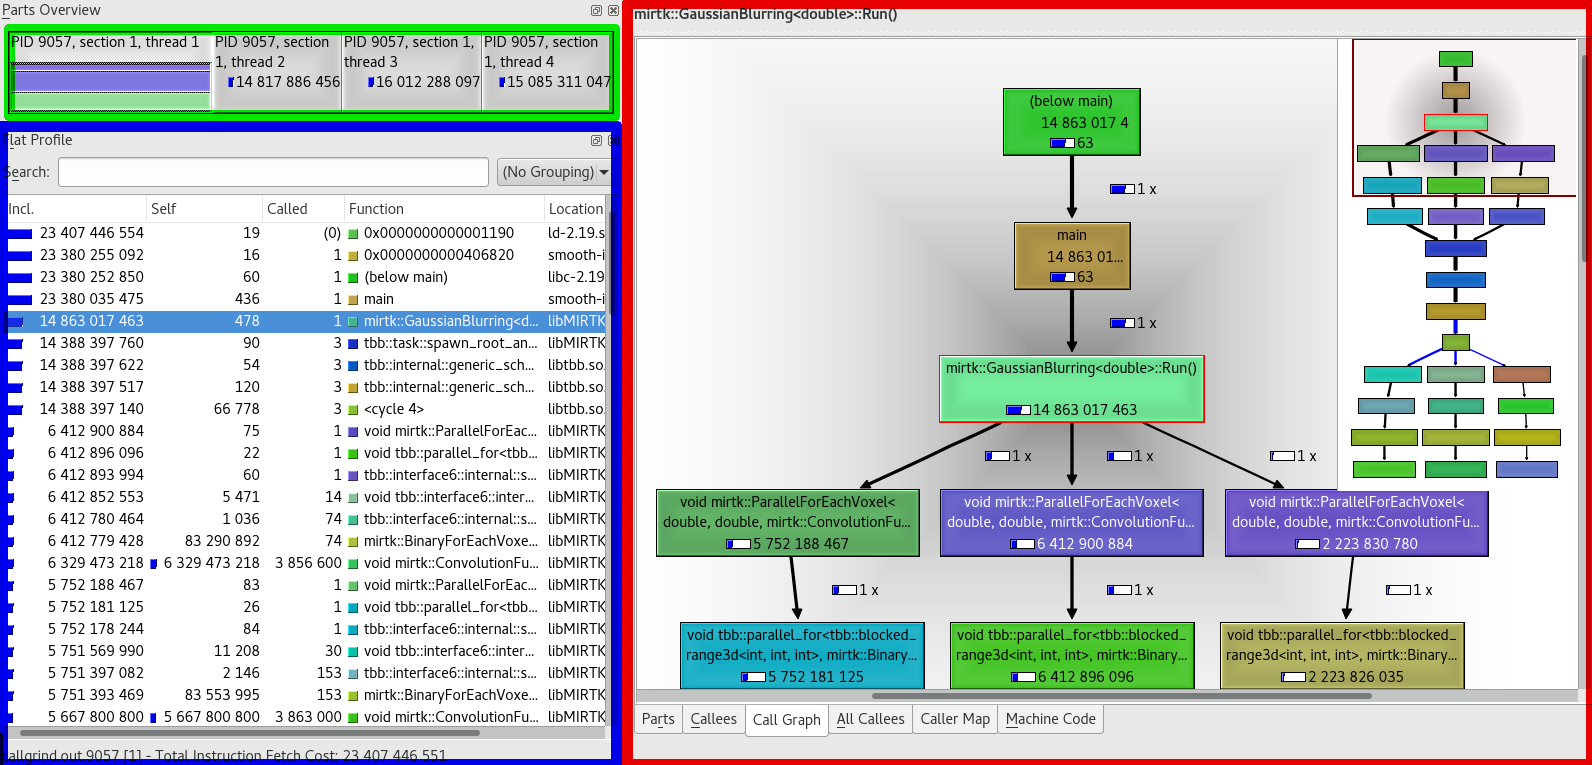
\includegraphics[width=13cm]{Reports/figures/UIkcachegrind.png}
%			\end{center}	
%			\caption{Interface de KCacheGrind pour le profilage}
%			\label{Interface de KCacheGrind pour le profilage}
%		\end{figure}~\par
%		{$\bullet$} \textit{Cadre vert: } Dans cette partie est distinguée tous les threads qui ont exécuté une partie du code lié à l'exécutable étudié. Tous les threads ayant été utilisés dans ce cas, on peut constater que la machine fonctionne donc avec 4 coeurs. \newline
%		{$\bullet$} \textit{Cadre bleu: } Ici est détaillé toutes les fonctions les plus coûteuses du thread sélectionné. \newline
%		{$\bullet$} \textit{Cadre rouge: } Grâce à ce diagramme, on peut visualiser la pile d'appel des fonctions avant et après la fonction sélectionné dans le cadre bleu. Les onglets en bas de page sont d'autres représentations plus textuelles (et plus détaillées) de ce que montre le diagramme. \newline
%		
%		
%	
%	%	=> on identifie les fonctions sur lesquelles agir en premier
%	%	On utilise Valgrind, qui, avec callgrind analyse la manière dont les caches sont utilisés.
%	%	Expliquer le choix de valgrind, parmi les autres profileurs
%	% => projet open-source multi-plateforme et disponible dans les packages linux, autres alternatives étudiées (VTUNE intel, installation compliquée, et codeXL, qui nécessite des proc AMD).\\
%		
%		
%	
%		
%		\paragraph{Analyse du nombre d'instructions}
%		
%		\begin{wrapfigure}{r}{7.2cm}
%			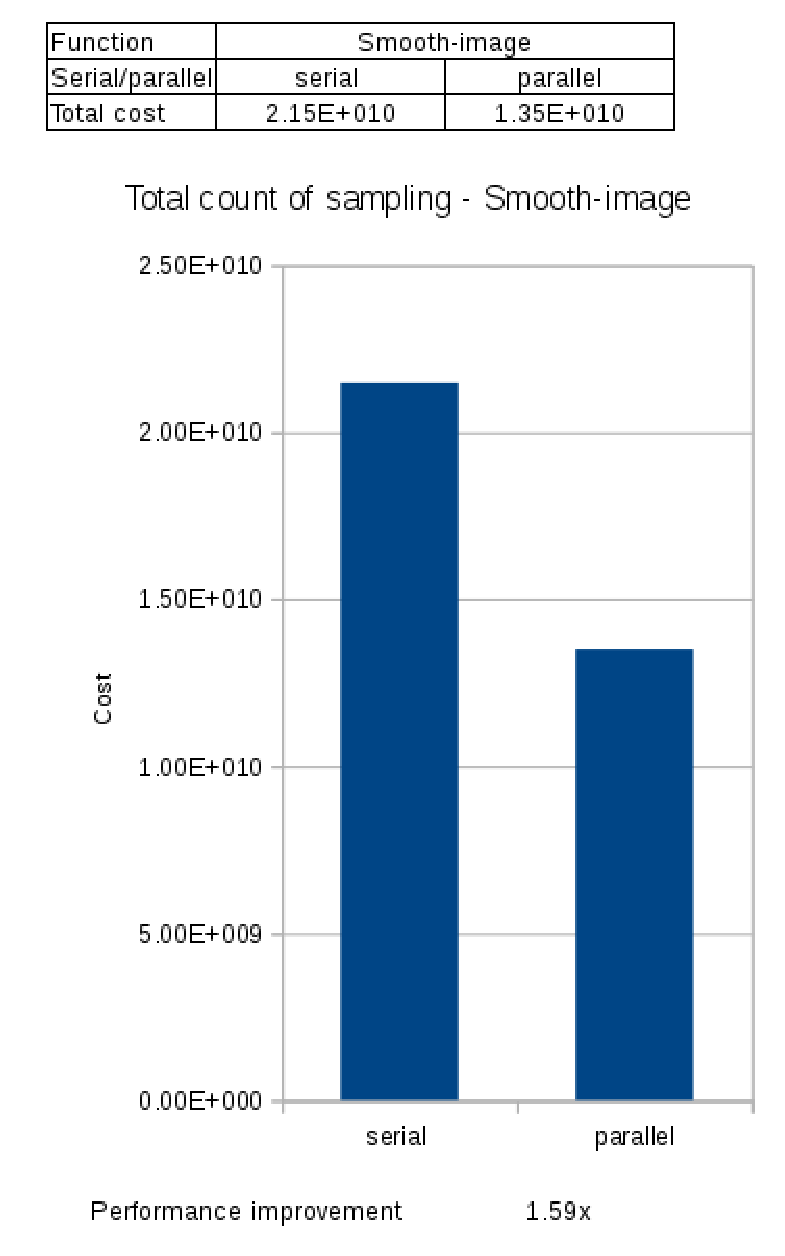
\includegraphics[height=9cm]{Reports/figures/smooth_image_costs.eps}
%			\caption{Coût de la fonction de flou gaussien}
%			\label{Coût de la fonction de flou gaussien}
%		\end{wrapfigure}
%		~\par~\par
%		Dans un premier temps, on s'intéresse au critère le plus pertinent concernant les performances du logiciel. Le nombre d'instructions correspond à la quantité de commandes atomiques (au niveau binaire) exécutées par le CPU et pour chaque thread.
%		Ainsi, on peut étudier l'efficacité de TBB en comparant le nombre d'instructions utilisées lorsque TBB est activé ou non. C'est ce qui est présenté sur l'image présentée ci-contre, en se focalisant sur une fonction de flou gaussien (nommée \textit{smooth-image}).\\
%		Sur l'axe des ordonnées, on a le coût total en instruction de la fonction, appelée sur une machine précise, avec une entrée précise (ici une image 3D). Les résultats dépendent de ces deux critères.Cependant, le ratio entre les coûts de la fonction parallélisée et celle qui ne l'est pas reste sensiblement le même. Au bas de l'image, on peut voir qu'ici, la fonction à un taux d'amélioration de x1.59. L'ordinateur ayant exécuté cette fonction ayant 8 coeurs, on peut dire que ce résultat reflète une mauvaise parallélisation dans ce cas, car un logiciel bien optimisé aurait un taux d'amélioration proche de x8 (équivalent au nombre de coeurs utilisés).\\
%		De même, ci-dessous, l'image décrit les performances de la fonction \textit{transform-image}. En revanche, ici, cette fonction possède une option qui permet de choisir son type d'interpolation mathématique. On a donc fait un test de coût d'instructions pour chaque interpolation et on a relevé ici le taux de performance associé:
%		\begin{figure}[h!]
%			\begin{center}
%				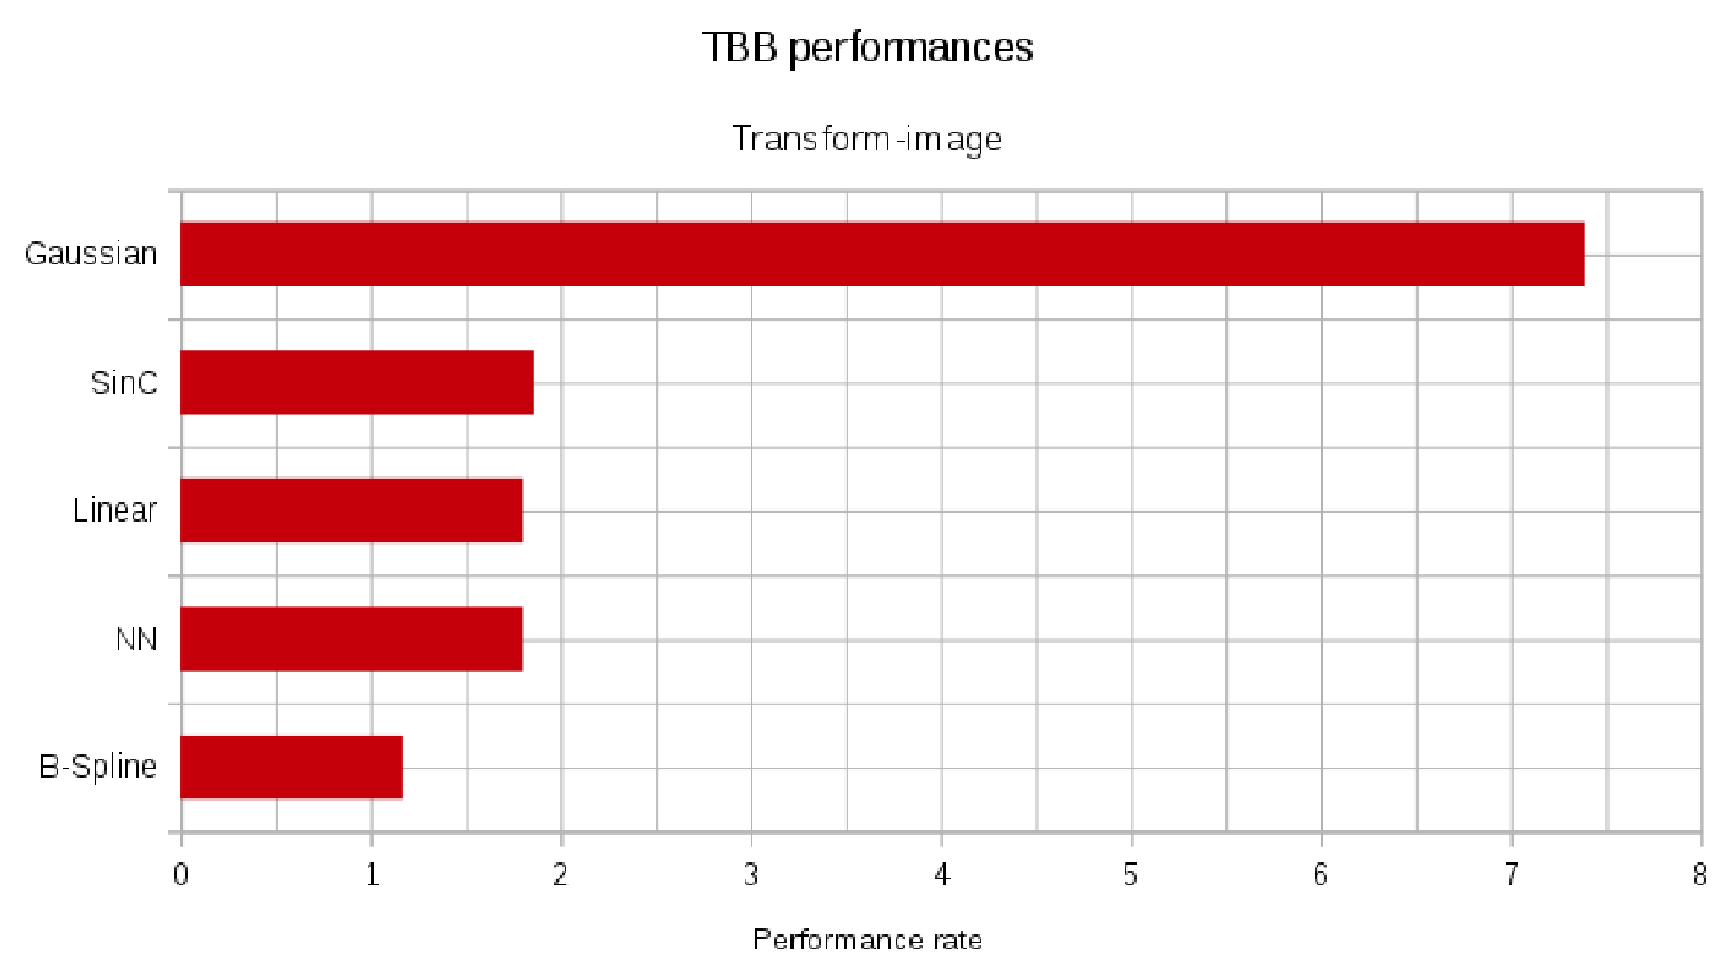
\includegraphics[width=9cm]{Reports/figures/performances_tbb_transform_image.eps}
%			\end{center}	
%			\caption{Améliorations apportées par TBB pour transform-image}
%			\label{Améliorations apportées par TBB pour transform-image}
%		\end{figure}~\par
%		L'interpolation gaussienne est donc parfaitement parallélisée, ce qui n'est pas le cas des autres interpolations de \textit{transform-image}.
%		
%		\paragraph{Analyse des fuites de cache}
%		Un deuxième critère intéressant à regarder, au travers du profilage, est la quantité de fuites de caches à l'exécution de la fonction étudiée. Bien que la parallélisation ne soit pas toujours optimale, elle peut néanmoins être parfois délaissée au profit d'une gestion de fuites de caches plus poussée.
%		
%		\subparagraph{Qu'est-ce qu'une fuite de cache?}
%		\textit{?????}\\
%		Ci-dessous est détaillé l'histogramme de la quantité des fuites de caches pour \textit{transform-image}, dans chaque mode d'interpolation:
%			\begin{figure}[h!]
%				\begin{center}
%					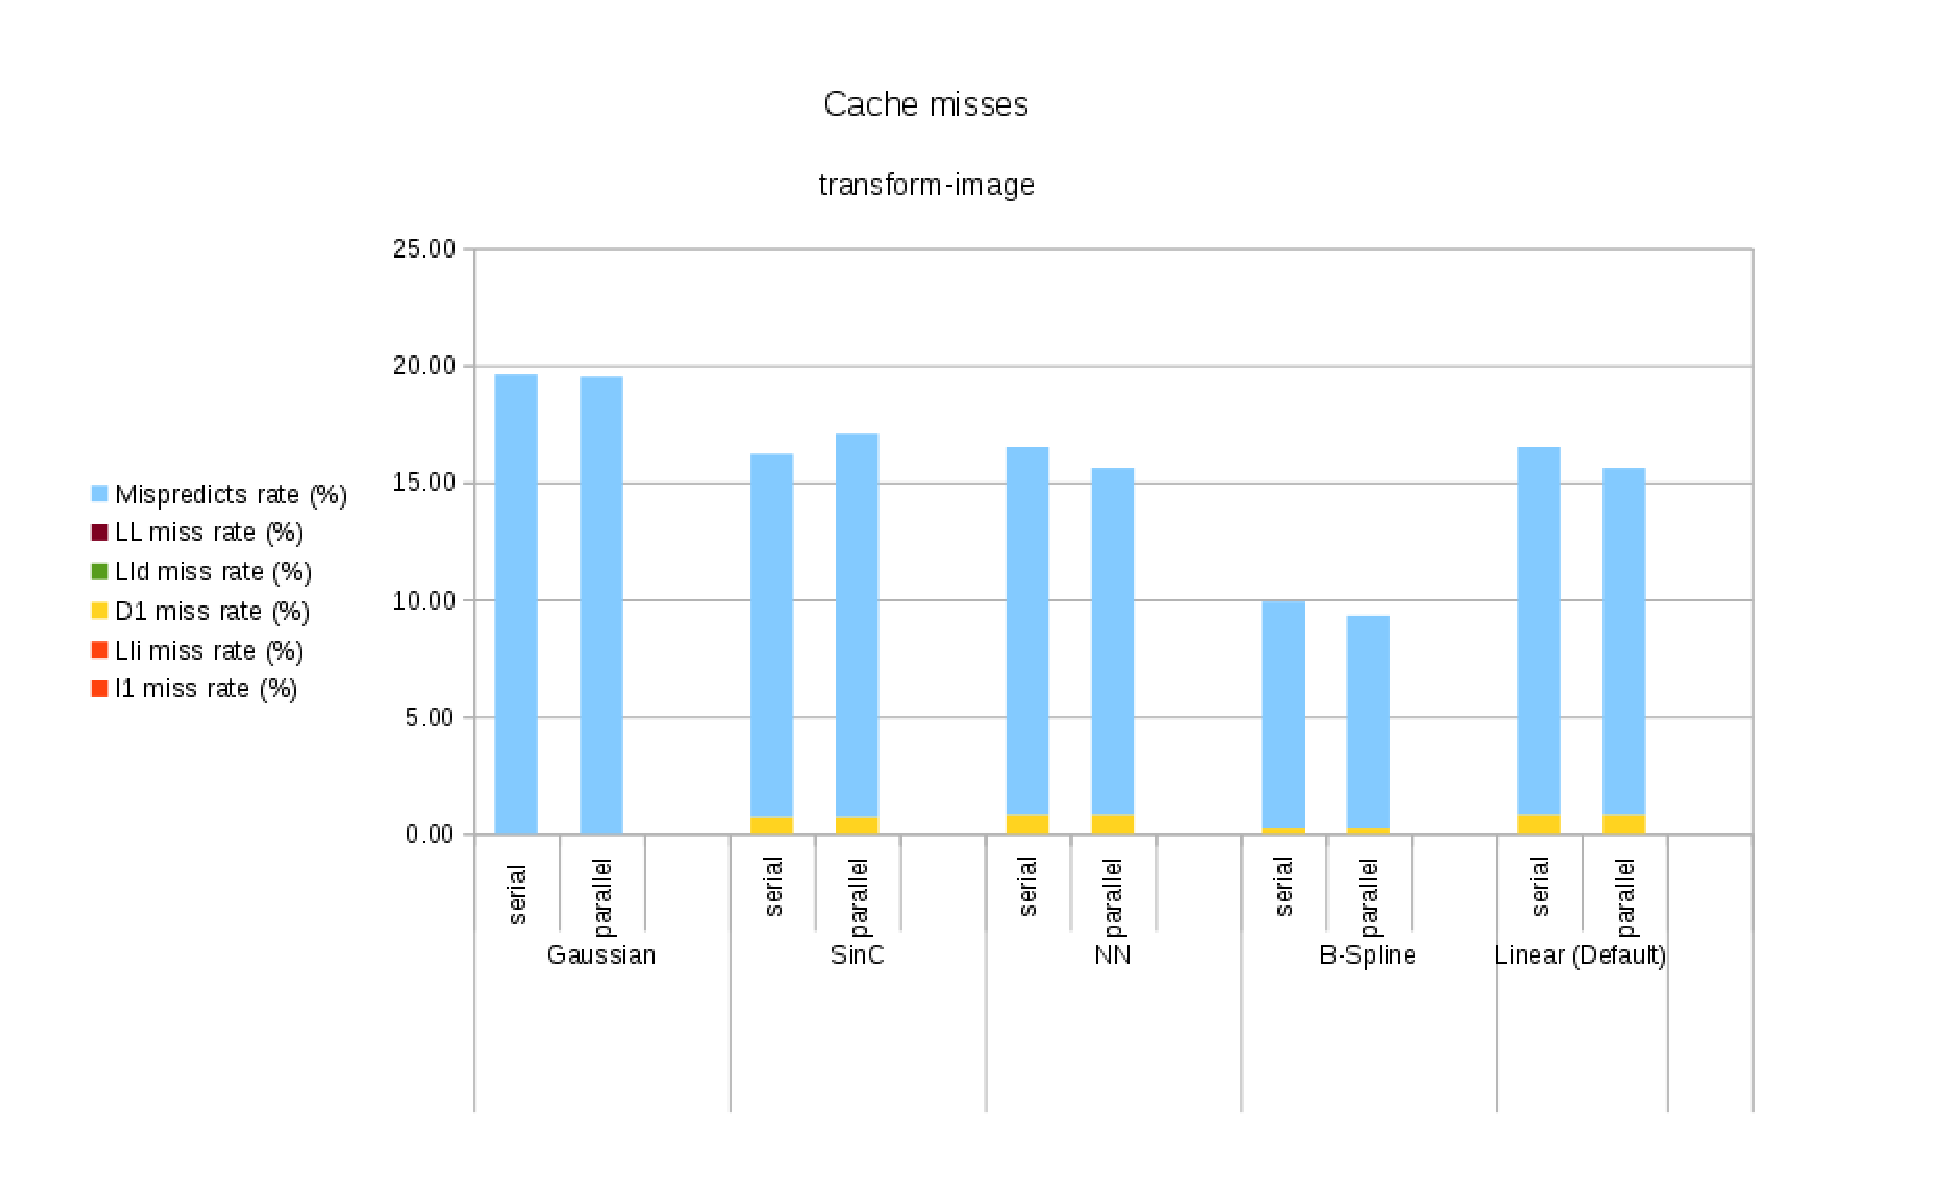
\includegraphics[width=15cm]{Reports/figures/cache_misses_transform_image.eps}
%				\end{center}	
%				\caption{Fuites de cache pour la fonction transform-image}
%				\label{Fuites de cache pour la fonction transform-image}
%			\end{figure}~\par
%		Les valeurs données ci-dessus (en pourcentage) sont assez mal réparties, mais le faible "cache miss rate" (taux de fuites de caches) est très faible. Le seul taux non négligeable est celui des mauvaises prédictions de branche, qui peut être considéré comme une fuite de cache, mais un taux inférieur à 20 \% reste négligeable. 
%		~\par
%		MIRTK est donc bien conçu au niveau de la gestion de la mémoire cache, alors que le système de parallélisation est largement améliorable.

%	\subsection{Switch automatique de back-end}
%	Commandes prépocesseur pour indiquer au logiciel quel est le back-end à utiliser (ArrayFire ou Eigen) en fonction de l'opération souhaitée.

	\subsection{Benchmarking}
%	(partie dépendante du déroulement du projet)\newline
%	- Analyse des performances obtenues \newline
%	- Comparaison avec le profilage initial ? \newline
%	- Points où il y a eu des concessions (exemple: alourdir le code pour parvenir à un résultat précis)
	
\chapter{Améliorations et perspectives}
	\section{A cours terme}
	\section{A long terme}

\chapter*{Conclusion} % dans cet ordre
\addcontentsline{toc}{chapter}{Conclusion}
\chapter*{Sources}
\addcontentsline{toc}{chapter}{Sources}
\noindent
\url{https://biomedia.doc.ic.ac.uk/}  : image page de garde, partie du texte 1.1.2 \\
\url{http://www.imperial.ac.uk} : partie du texte 1.1.1 (Department of computing) et schéma stratégie du département\\
\url{https://fr.wikipedia.org/wiki/Imperial_College_London} : partie du texte 1.1.1 (Imperial College London)\\
\url{http://ric.uthscsa.edu/mango/papaya/index.html} : outil de visualisation d'images en format NIFTI
\renewcommand{\listfigurename}{Table des illustations}
\listoffigures
\addcontentsline{toc}{chapter}{Table des illustrations}
\chapter*{Glossaire}
\addcontentsline{toc}{chapter}{Glossaire}
\noindent
\textbf{Back-end:}\\ 
\textbf{Front-end:}\\
\textbf{MIRTK:}\\
\textbf{Profilage:} Différence avec le benchmarking ?\\
\textbf{Run-time:}\\
\textbf{Fuite de cache:}\\
\textbf{Benchmarking:} Différence avec le profiling ?\\
\textbf{Thread:}\\
\textbf{Prédiction de branche:}\\
\textbf{Fuite de cache:}\\


\definecolor{mygreen}{rgb}{0,0.6,0}
\definecolor{mygray}{rgb}{0.5,0.5,0.5}
\definecolor{mymauve}{rgb}{0.58,0,0.82}

\lstset{ %
	backgroundcolor=\color{white},   % choose the background color
	basicstyle=\footnotesize,        % size of fonts used for the code
	breaklines=true,                 % automatic line breaking only at whitespace
	captionpos=b,                    % sets the caption-position to bottom
	commentstyle=\color{mygreen},    % comment style
	escapeinside={\%*}{*)},          % if you want to add LaTeX within your code
	keywordstyle=\color{blue},       % keyword style
	stringstyle=\color{mymauve},     % string literal style
}

\begin{appendix}
	\chapter*{Annexe 1: Implémentation de "smooth-image" en Python}
	\addcontentsline{toc}{chapter}{Annexe 1: Implémentation de "smooth-image" en Python}
	\begin{lstlisting}[language=python]
import arrayfire as af
from array import array
import matplotlib.pyplot as plt
import nibabel as nib 
from scipy import signal
from scipy.fftpack import fft, fftshift 
import numpy as np
import argparse as ap

if __name__ == '__main__':
	
	# Command line arguments and options handling 
	parser = ap.ArgumentParser()
	parser.add_argument("InputImage", type=str, help="Path to the input image")
	parser.add_argument("OutputImage", type=str, help="Path to the input image")
	parser.add_argument("Sigma", type=int, help="Defines the value of sigma for the Gaussian kernel. Default: 1")
	parser.add_argument("--dimension", type=str, choices=["x", "y", "z", "xy", "yz", "xz", "xyz"], help="Specifies on which dimensions execute the blurring. Default: xyz")
	parser.add_argument("-color", help="Enable colored input/output image plot.", action="store_false")
	parser.add_argument("-nodisplay", help="Cancel plot of the input/output images. Has priority over \"-color argument\".", action="store_false")
	
	args = parser.parse_args()
	
	# Loading input
	img = nib.load(args.InputImage)
	hdr = img.get_header()
	img_data = img.get_data().astype('f')
	
	# Conversion numpy => arrayfire
	img_data_af = af.interop.np_to_af_array(img_data)
	
	# Declaration of Gaussian kernel
	if args.Sigma:
		kernel = signal.gaussian(img_data.shape[0], std = args.Sigma).astype('f')
	else:
		kernel = signal.gaussian(img_data.shape[0], std = 1).astype('f')
	
	# Conversion numpy => arrayfire for the Gaussian kernel
	kernel_af = af.interop.np_to_af_array(kernel)
	
	# Convolution along dimensions chosen 
	output_image = img_data_af.copy()
	input_image = img_data_af.copy()
	
	if (args.dimension):
	
		if ("x" in args.dimension):
			output = af.convolve1(input_image, kernel_af)
		
		if ("y" in args.dimension):
			input_image = af.reorder(output_image, 1, 0, 2)
			output_image = af.convolve1(input_image, kernel_af)
			output_image = af.reorder(output_image, 1, 0, 2)
		
		if ("z" in args.dimension):
			input_image = af.reorder(output_image, 2, 1, 0)
			output_image = af.convolve1(input_image, kernel_af)
			output_image = af.reorder(output_image, 2, 1, 0)
	else:
		output_image = af.convolve1(input_image, kernel_af)
		input_image = af.reorder(output_image, 1, 0, 2)
		output_image = af.convolve1(input_image, kernel_af)
		output_image = af.reorder(output_image, 1, 0, 2)
		input_image = af.reorder(output_image, 2, 1, 0)
		output_image = af.convolve1(input_image, kernel_af)
		output_image = af.reorder(output_image, 2, 1, 0)
	
	
	# Conversion arrayfire => numpy
	output_np = output_image.to_array()
	output_np = np.asarray(output_np)
	output_np = output_np.reshape(320, 250, 202, order='F')
	
	# Saving the output file
	affine = img.get_affine()
	new_img = nib.Nifti1Image(output_np, affine)
	nib.save(new_img, args.OutputImage)
	
	# Check if plot is not cancelled by "-nosdisplay" argument
	if (args.nodisplay == True):
		# Assimilating color option
		if (args.color):
		colors = 'gray'
		else:
		colors = None
		
		# Ploting 1rst window
		f,fig = plt.subplots(1, 2)
		fig[0].imshow(img_data[125, :, :].T, extent=[0, hdr['pixdim'][1], 0, hdr['pixdim'][3]], cmap=colors, origin='lower')
		fig[1].imshow(output_np[125, :, :].T, extent=[0, hdr['pixdim'][1], 0, hdr['pixdim'][3]], cmap=colors, origin='lower')
		plt.suptitle("Gaussian Blurring on x-axis")
		
		# Ploting 2nd window
		f2,fig2 = plt.subplots(1, 2)
		fig2[0].imshow(img_data[:, 125, :].T, extent=[0, hdr['pixdim'][1], 0, hdr['pixdim'][3]], cmap=colors, origin='lower')
		fig2[1].imshow(output_np[:, 125, :].T, extent=[0, hdr['pixdim'][1], 0, hdr['pixdim'][3]], cmap=colors, origin='lower')
		plt.suptitle("Gaussian Blurring on y-axis")
		
		# Ploting 3rd window
		f3,fig3 = plt.subplots(1, 2)
		fig3[0].imshow(img_data[:, :, 125].T, cmap=colors, origin='lower')
		fig3[1].imshow(output_np[:, :, 125].T, cmap=colors, origin='lower')
		plt.suptitle("Gaussian Blurring on z-axis")
		
		plt.show()
	\end{lstlisting}
\end{appendix}

\end{document}
